\chapter{Experiments}
\label{ch:intro}

In order to evaluate our extension of ILP, the correlation and lattice, and the different interestingness measures, we
perform a series of experiments on Linked Data.

First, we test our proposed approach on LinkedMDB and DBpedia. We merge both datasets onto a single RDF3X database,
create correlation lattices for the properties $budget$ and $runtime$ with categorical relations: $director$,
$writer$, $producer$, $distributor$, $starring$, $country$, and $subject$. We build a pair lattices for each of the 4
interestingness measures we evaluate: Kullback-Leibler divergence only, Kullback-Leibler combined with support,
Jensen-Shannon combined with support, and support only

Subsequently, we run the ILP with our proposed extension and learn rules with the relation $country$ as head. We
measure the number of base-rules evaluated as interesting, the runtime spent with their search, and how many of the
rules evaluated as interesting actually had an interesting refined-rule. It is important to point out that the
core-ILP runtime, excluding the search for rules with numerical intervals, is the same for all of them measures and
threshold values. 

This is done for the 4 aforementioned measures and various different threshold values. With that we can obtain evaluate
the accuracy and recall of our interestingness predictions, as well as evaluate their efficiency by comparing the amount
of rules learned per runtime.

In this experiment, we used equal frequencies as discretization technique, since the numerical properties are skewed and
quite noisy, with the property $budget$, for instance, containing significant outliers with order of magnitude up to
$10^{14}$.

Firstly, we compare different measures by building same-sized correlation lattices on the $hasIncome(X,Y)$
relation from the USCensus, then searching for interesting rules with intervals for $Y$ inside the lattice itself as
described in Section~\ref{sec:searchRulesInCL}. The lattices are build by greedily choosing the top-k most interesting
nodes in each level according to the chosen measure, and pruning the rest so that all the lattices have the same
quantity of nodes.

Also, we measure the total time spent for the construction of each lattice as well as the number of interesting rules
found in it. As candidate categorical relations, we chose the 18 shown in Table~\ref{tab:uscensusRelations}. More
details about the categories can be found at the PUMS
Data
Dictionary\footnote{\url{http://www.census.gov/acs/www/Downloads/data_documentation/pums/DataDict/PUMSDataDict05_07.pdf}
}

\begin{table}[h!]
\begin{minipage}{\textwidth}
 \begin{center}
 \caption{Chosen categorical relations from USCensus}
  \begin{tabular}{l l c}
    \toprule
      Name	& Label				& Number of Categories \\
    \midrule
      sex	& Sex				&	2	\\
      st	& State				&	52\footnote{Including Puerto Rico and Washington D.C.}	\\
      racwht	& is White			&	2	\\
      racblk	& is Black			&	2	\\
      racasn	& is Asian			&	2	\\
      qtrbir	& Quarter of Birth		&	4	\\	
      nativity	& born In the US		&	2	\\
      mar	& Marital Status		&	5	\\
      lanp	& Language Spoken at Home	&	104	\\
      esr	& Employment Status		&	6	\\
      dphy	& Physical Difficulty		&	2	\\
      schl	& Educational Level		&	17	\\	
      occp	& Occupation			&	470	\\
      sch	& School Enrollment		&	3	\\
      rel	& Relationship (to household owner)		&	12	\\
      esp	& Employment Status of Parents	&	8	\\
      oc	& Own Child			&	2	\\
    \bottomrule
  \end{tabular}
 \label{tab:uscensusRelations}
 \end{center}
\end{minipage}
\end{table}

The plot from Figure~\ref{fig:uscensus:Nodes-GoodRules} shows the number of rules learned per lattice size (defined by
number of nodes per level). As observed, 


Since the USCensus data is completely joined on person entities, and all categorical relations have literals
as constants (usually integer numbers mapped to a set of entities), therefore allowing only star-join patterns, we
chose DBpedia and LinkedMDB in order to evaluate our ILP-extension.


\begin{figure}
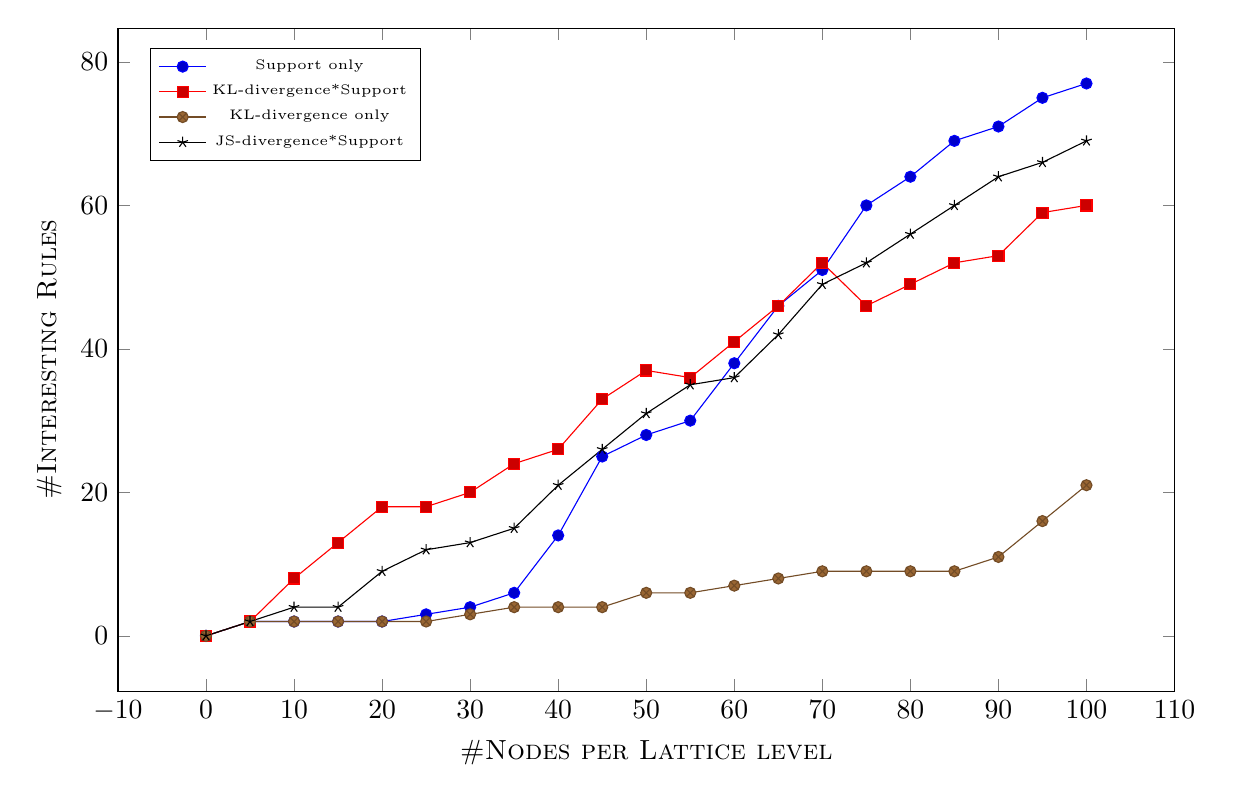
\begin{tikzpicture}[scale=1.0]
 \begin{axis}[
	width=15cm, height=10cm,
        xlabel=\textsc{\#Nodes per Lattice level},
        ylabel=\textsc{\#Interesting Rules},
        legend entries={Support only, KL-divergence*Support, KL-divergence only, JS-divergence*Support},
	legend style={legend pos=north west,font=\tiny}]
    ]
% Support
\addplot coordinates {(0,0) (5,2) (10,2) (15,2) (20,2) (25,3) (30,4) (35,6) (40,14) (45,25) (50,28) (55,30) (60,38)
(65,46) (70,51) (75,60) (80,64) (85,69) (90,71) (95,75) (100,77)};
% KLDiv*Support
\addplot coordinates {(0,0) (5,2) (10,8) (15,13) (20,18) (25,18) (30,20) (35,24) (40,26) (45,33) (50,37) (55,36) (60,41)
(65,46) (70,52) (75,46) (80,49) (85,52) (90,53) (95,59) (100,60)};
% KLDiv Only
\addplot coordinates {(0,0)  (5,2) (10,2) (15,2) (20,2) (25,2) (30,3) (35,4) (40,4) (45,4) (50,6) (55,6) (60,7) (65,8)
(70,9) (75,9) (80,9) (85,9) (90,11) (95,16) (100,21)};
% JS*Support
\addplot coordinates {(0,0)  (5,2) (10,4) (15,4) (20,9) (25,12) (30,13) (35,15) (40,21) (45,26) (50,31) (55,35) (60,36)
(65,42) (70,49) (75,52) (80,56) (85,60) (90,64) (95,66) (100,69)};
\end{axis}
\end{tikzpicture}
\label{fig:uscensus:Nodes-GoodRules}
\end{figure}

\begin{figure}
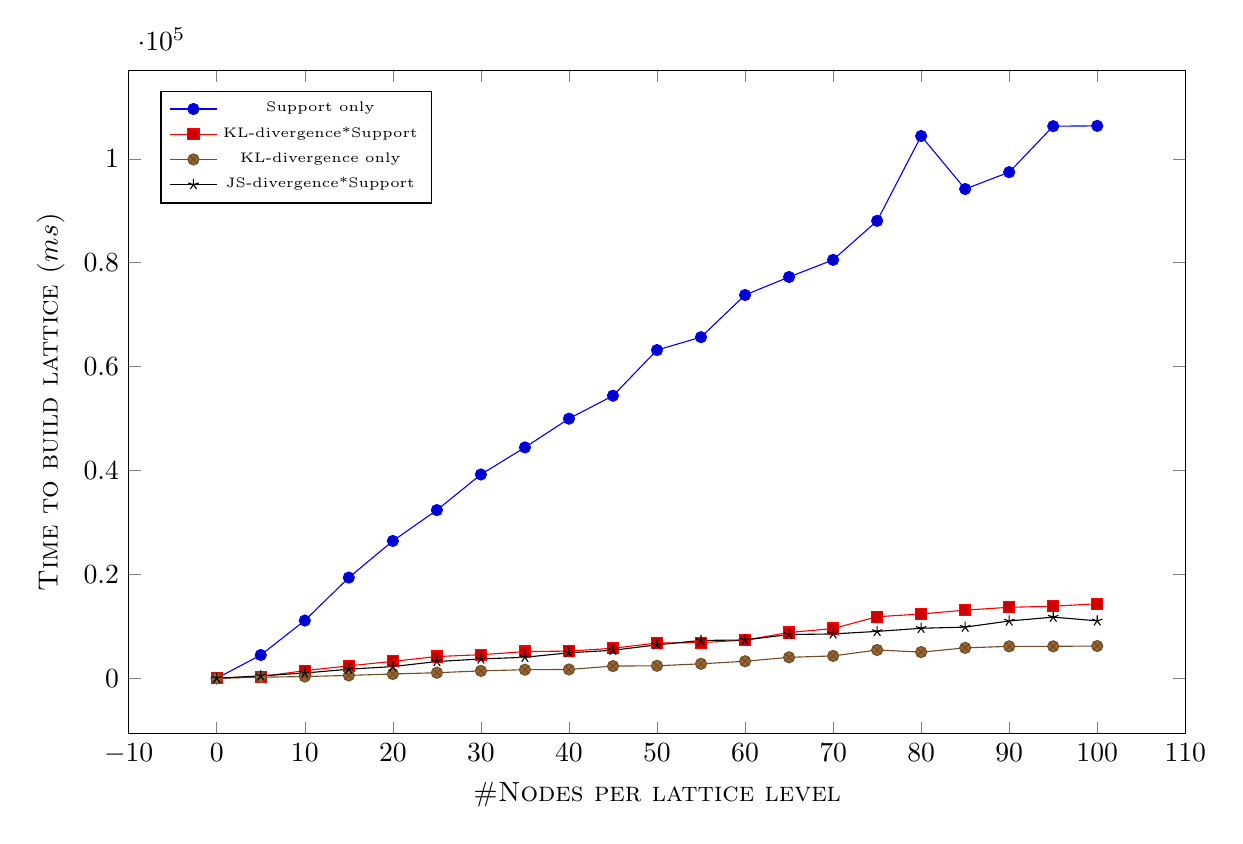
\begin{tikzpicture}[scale=1.0]
 \begin{axis}[
	width=15cm, height=10cm,
        xlabel=\textsc{\#Nodes per lattice level},
        ylabel=\textsc{Time to build lattice ($ms$)},
        legend entries={Support only, KL-divergence*Support, KL-divergence only, JS-divergence*Support},
	legend style={legend pos=north west,font=\tiny}]
    ]
\addplot coordinates {(0,0) (5,4471) (10,11113) (15,19383) (20,26432) (25,32374) (30,39228) (35,44439) (40,49974)
(45,54391) (50,63178) (55,65673) (60,73782) (65,77245) (70,80542) (75,88055) (80,104386) (85,94183) (90,97424)
(95,106279) (100,106336)};
\addplot coordinates {(0,0)  (5,321) (10,1463) (15,2390) (20,3253) (25,4184) (30,4529) (35,5137) (40,5231) (45,5774)
(50,6786) (55,6864) (60,7347) (65,8813) (70,9567) (75,11844) (80,12372) (85,13119) (90,13659) (95,13859) (100,14353)};
\addplot coordinates {(0,0)  (5,207) (10,329) (15,549) (20,825) (25,1065) (30,1420) (35,1652
) (40,1695) (45,2343) (50,2402) (55,2782) (60,3273) (65,4031) (70,4299) (75,5448) (80,5035) (85,5847) (90,6145)
(95,6146) (100,6208)};
\addplot coordinates {(0,0)  (5,466) (10,1011) (15,1746) (20,2253) (25,3220) (30,3717) (35,4042) (40,4904) (45,5390)
(50,6436) (55,7280) (60,7371) (65,8412) (70,8535) (75,9025) (80,9624) (85,9845) (90,11027) (95,11772) (100,11050)};
\end{axis}
\end{tikzpicture}
\label{fig:uscensus:Nodes-Runtime}
\end{figure}

\begin{figure}
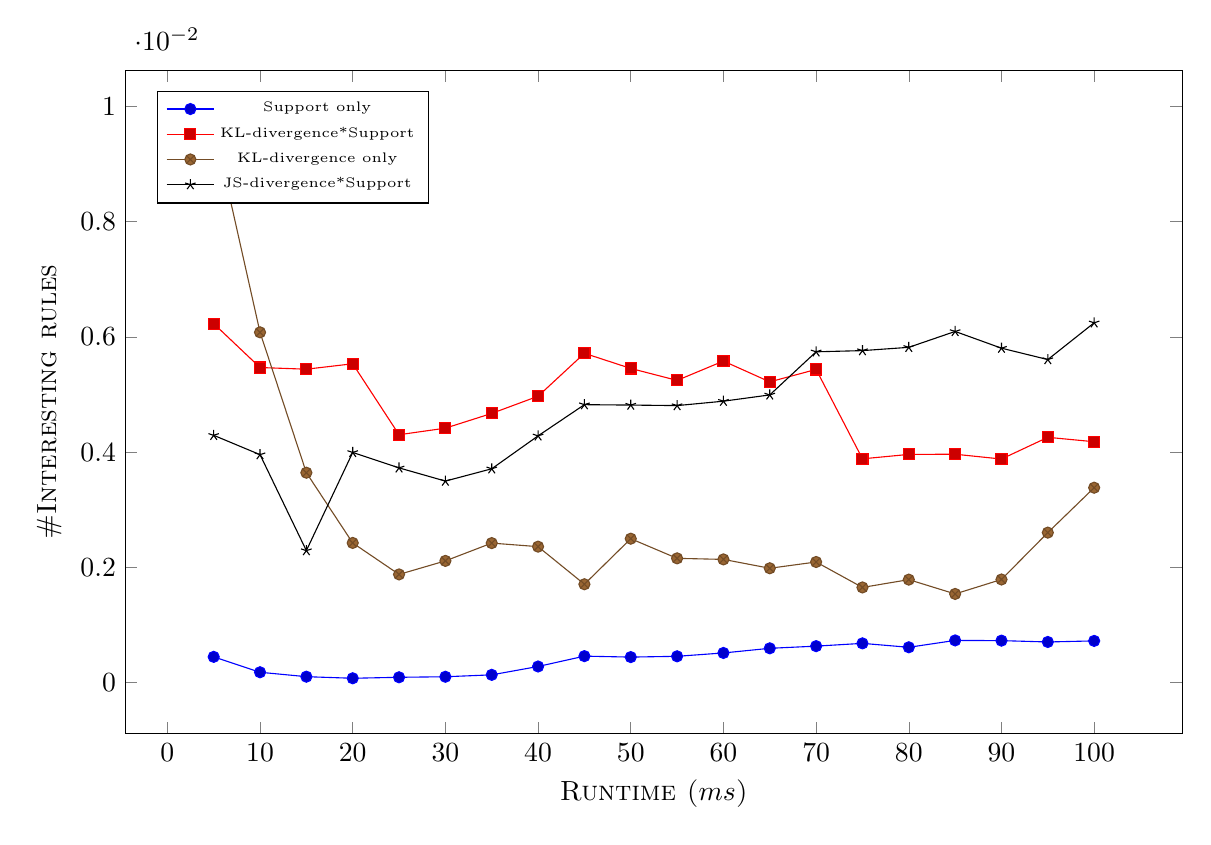
\begin{tikzpicture}[scale=1.0]
 \begin{axis}[
	width=15cm, height=10cm,
        xlabel=\textsc{Runtime ($ms$)},
        ylabel=\textsc{\#Interesting rules},
        legend entries={Support only, KL-divergence*Support, KL-divergence only, JS-divergence*Support},
	legend style={legend pos=north west,font=\tiny}]
    ]
\addplot coordinates {(5,0.0004473272) (10,0.0001799694) (15,0.0001031832) (20,7.566586e-05) (25 ,
9.266695e-05) (30,0.0001019680) (35,0.0001350165) (40,0.0002801457) (45,0.0004596349) (50 ,
0.0004431923) (55,0.0004568087) (60,0.0005150308) (65,0.0005955078) (70,0.00063321) (75,0.0006813923
) (80,0.000613109) (85,0.0007326163) (90,0.0007287732) (95,0.0007056897) (100,0.0007241198)};
\addplot coordinates {(5,0.00623053) (10,0.005468216) (15,0.005439331) (20,0.005533354) (25 ,
0.004302103) (30,0.004415986) (35,0.004671988) (40,0.004970369) (45,0.005715275) (50,0.005452402) (
55,0.005244755) (60,0.005580509) (65,0.005219562) (70,0.005435351) (75,0.003883823) (80 ,
0.003960556) (85,0.003963717) (90,0.003880225) (95,0.004257161) (100,0.004180311)};
\addplot coordinates {(5,0.009661836) (10,0.006079027) (15,0.003642987) (20,0.002424242) (25 ,
0.001877934) (30,0.002112676) (35,0.002421308) (40,0.002359882) (45,0.001707213) (50,0.002497918) (
55,0.002156722) (60,0.002138711) (65,0.001984619) (70,0.00209351) (75,0.001651982) (80,0.001787488
) (85,0.001539251) (90,0.001790073) (95,0.002603319) (100,0.003382732)};
\addplot coordinates {(5,0.004291845) (10,0.003956479) (15,0.002290951) (20,0.003994674) (25 ,
0.003726708) (30,0.003497444) (35,0.003711034) (40,0.004282219) (45,0.004823748) (50,0.004816656) (
55,0.004807692) (60,0.004884005) (65,0.004992867) (70,0.005741066) (75,0.005761773) (80 ,
0.005818786) (85,0.006094464) (90,0.005803936) (95,0.005606524) (100,0.006244344)};
\end{axis}
\end{tikzpicture}
\end{figure}


\begin{figure}
 \caption{Precision - Recall }
 \centering
 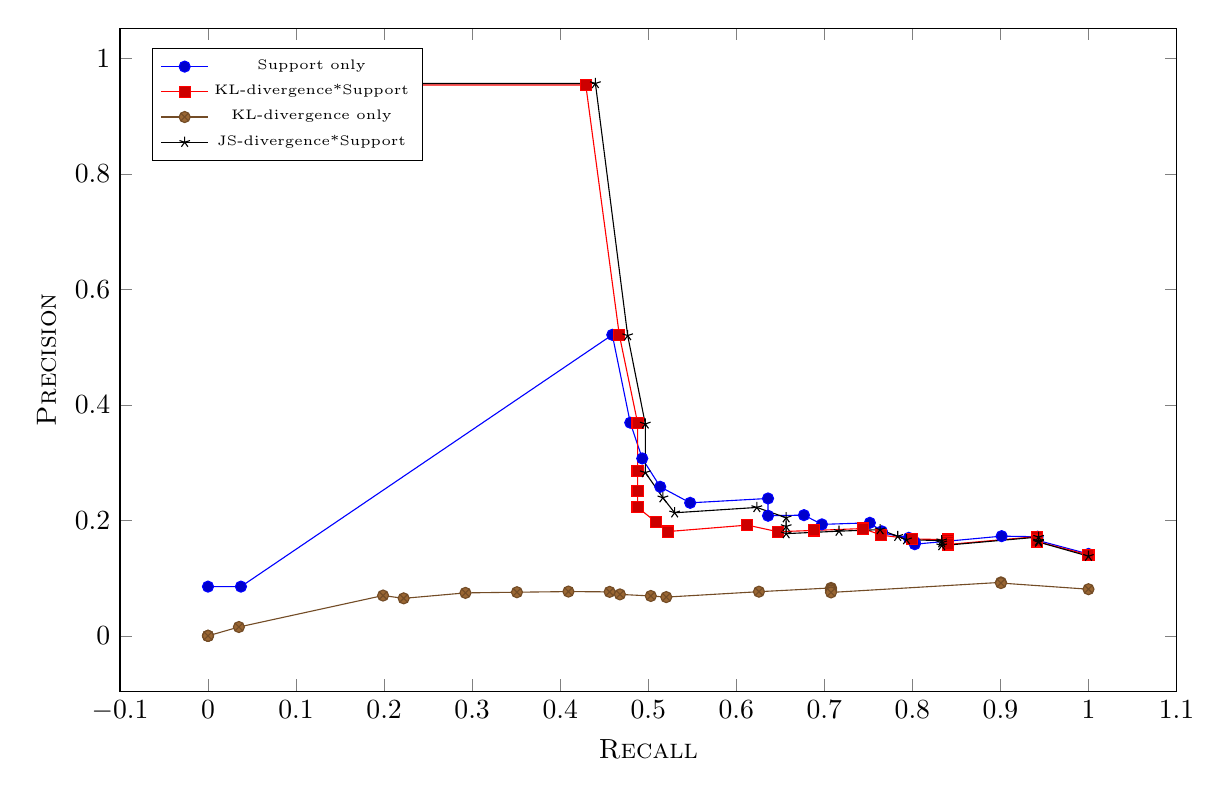
\begin{tikzpicture}[scale=1.0]
  \begin{axis}[
	width=15cm, height=10cm,
	xlabel=\textsc{Recall},
	ylabel=\textsc{Precision},
	legend entries={Support only, KL-divergence*Support, KL-divergence only, JS-divergence*Support},
	legend style={legend pos=north west,font=\tiny}]
      ]
  \addplot coordinates {(0,0.08527132) (0.03741496,0.08527132) (0.4591837,0.5212355) (0.4795918,0.3691100)
(0.4931973,0.3072034)
(0.5136054,0.2581197) (0.547619,0.2303290) (0.6360544,0.2379135) (0.6360544,0.2080089) (0.6768708,0.2090336)
(0.6972789,0.193032) (0.7517007,0.1957484) (0.7653061,0.1810137) (0.7653061,0.1781473) (0.7959183,0.1696882)
(0.8027211,0.1621993) (0.8027211,0.1587088) (0.9013606,0.1726384) (0.9421769,0.1716233) (0.9421769,0.1653731)
(1.0,0.1418234)};

   \addplot coordinates { (0,0.9538462) (0.4290657,0.9538462) (0.467128,0.5212355) (0.4878893,0.3691100)
(0.4878893,0.2848485) (0.4878893,0.2508897) (0.4878893,0.2227488) (0.5086505,0.1970509) (0.5224913,0.180622)
(0.6124567,0.1917660) (0.6470588,0.1803279) (0.6885813,0.1825688) (0.7439446,0.1858254) (0.7647059,0.1744278)
(0.799308,0.1676343) (0.8408305,0.1667810) (0.8408305,0.1631968) (0.8408305,0.1583062) (0.9411765,0.1718256)
(0.9411765,0.1654501) (0.9411765,0.1634615) (1.0,0.1401552)};

  \addplot coordinates {(0,0) (0,0) (0,0) (0,0) (0.03508772,0.01530612) (0.1988304,0.0698152) 
  (0.2222222,0.06495727) (0.2923977,0.07440476) (0.3508772,0.07556675) (0.4093567,0.07667032) (0.4561403,0.07617188)
(0.4678363,0.07181329) (0.502924,0.06907631) (0.5204678,0.06711916) (0.625731,0.0764832) (0.7076023,0.0829904)
(0.7076023,0.0810992) (0.7076023,0.07846952) (0.7076023,0.07520199) (0.9005848,0.09260373)
 (0.9005848,0.09139466) (1.0,0.08077468)};

 \addplot coordinates {(0,0.9565217) (0.44,0.9565217) (0.4766667,0.52) (0.4966667,0.3669951) 
(0.4966667,0.2827325) (0.5166667,0.2391975) (0.53,0.2131367) (0.6233333,0.2223543) (0.6566667,0.2045691)
 (0.6566667,0.1894231) (0.6566667,0.1769991) (0.7166666,0.1812816) (0.7633333,0.1839358) (0.7833334,0.1724138)
 (0.7933334,0.1665500) (0.8333333,0.1649076) (0.8333333,0.1612903) (0.8333333,0.15625) (0.9433333,0.1711004) 
 (0.9433333,0.1644393) (0.9433333,0.1623637) (1.0,0.1379310)};


  \end{axis}
  \end{tikzpicture}
\end{figure}

\begin{figure}
 \caption{Runtime-LearnedRules}
 \centering
 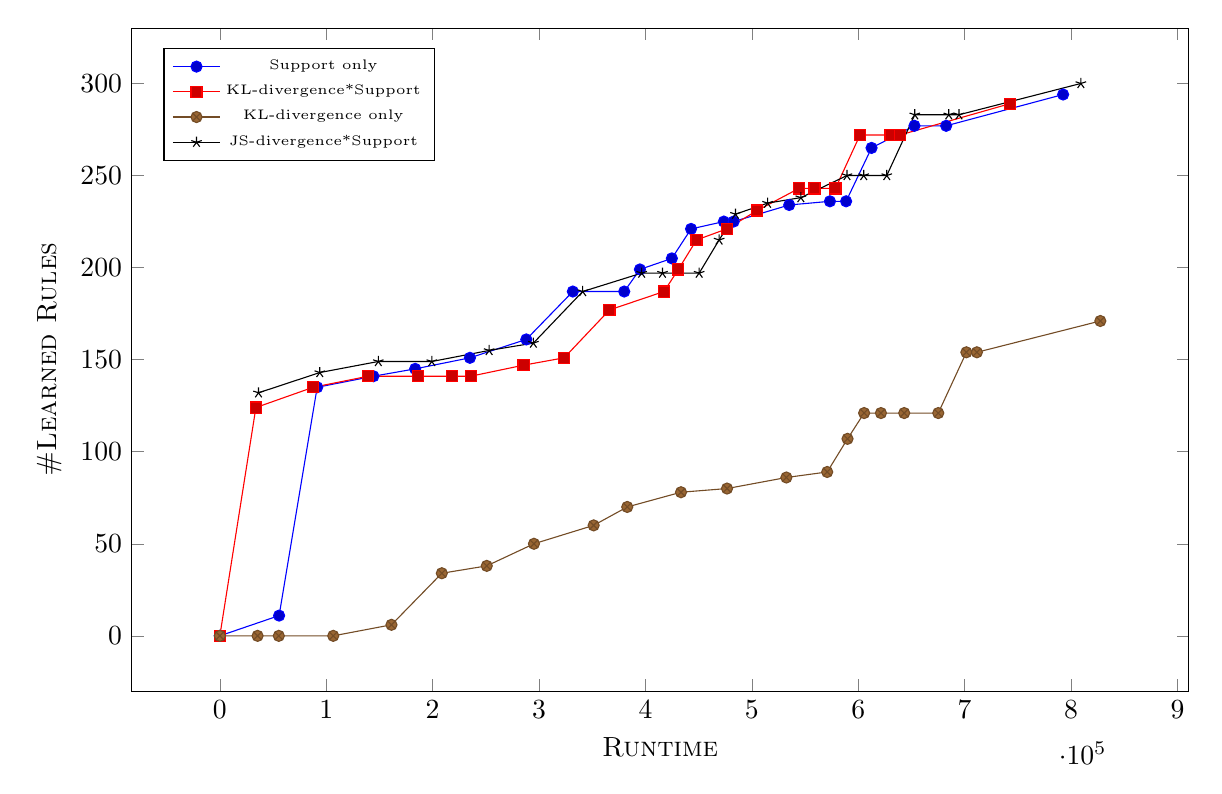
\begin{tikzpicture}[scale=1.0]
  \begin{axis}[
	width=15cm, height=10cm,
	xlabel=\textsc{Runtime},
	ylabel=\textsc{\#Learned Rules},
        legend entries={Support only, KL-divergence*Support, KL-divergence only, JS-divergence*Support},
	legend style={legend pos=north west,font=\tiny}]
      ]
  \addplot coordinates {(0.0,0.0) (55709,11) (91488,135) (144319,141) (183567,145) (235053,151) (288040,161)
(331747,187)
(380080,187) (394814,199)
(424827,205) (442860,221) (473691,225) (482918,225) (535099,234) (573386,236) (588600,236) (612505,265) (652833,277)
(682636,277) (792557,294)};

  \addplot coordinates {(0.0,0.0) (33892,124) (87747,135) (139353,141) (186294,141) (217893,141) (235750,141)
(285443,147)
(323626,151) (366197,177) (417438,187) (430932,199) (447970,215) (476371,221) (504948,231) (544307,243) (558897,243)
(578569,243) (601647,272) (630384,272) (639120,272) (742514,289)};
 
  \addplot coordinates {(0.0,0.0) (35466,0.0) (55421,0.0) (106586,0.0) (161302,6) (208629,34) (250863,38) (295212,50)
(351300,60)
(382899,70) (433423,78) (476677,80) (532442,86) (570818,89) (589925,107) (605518,121) (621333,121) (643190,121)
(675208,121) (701631,154) (711515,154) (827520,171)};

 \addplot coordinates { (36343,132) (93944,143) (148944,149) (199223,149) (253104,155) (294678,159) (341024,187)
(396459,197) (416000,197) (450504,197) (469231,215) (484591,229) (514785,235) (546069,238) (589417,250) (605128,250)
(626821,250) (653140,283) (685085,283) (694687,283) (809238,300)};

  \end{axis}
  \end{tikzpicture}
\end{figure}


\subsection{Example of Rules Learned}

We selected a couple of interesting rules learned with our approach in order to illustrate the kind of results we
obtain. On LinkedMDB, for example, we learned that films in English with Canadian director, and low budget are
significantly more likely to be also Canadian than those with higher budget. The base rule shown below has
confidence $0.36$:

$country(X,canada)$ :- $director(X,Z),bornIn(Z,canada),language(X,english),budget(X,Y)$

When we refine this rule, we find an interval with confidence $0.83$:

$country(X,canada)$ :- $director(X,Z),bornIn(Z,canada),language(X,english),budget(X,Y),Y\leq 80000$

Another interesting example reveals that films written by a spouse of Fritz Lang (in this case, Thea von
Harbou, who was an actress, writer, and director), and which have long runtime are more likely to have been directed by
Fritz Lang than those with shorter runtime. The base rule has confidence $0.6$:

$director(X,fritzLang)$ :- $writer(A,D),spouse(D,fritzLang),runtime(X,Y)$

And the refined rule has confidence $0.82$:

$director(X,fritzLang)$ :- $writer(A,D),spouse(D,fritzLang),runtime(X,Y),Y\geq 6800s$

Other examples of interesting rules learned are shown in Table~\ref{tab:mdbRuleExamples}.

\begin{table}[h!]
\begin{minipage}{\textwidth}
 \begin{center}
 \caption{Interesting rules with numerical intervals learned from DBpedia}
  \begin{tabular}{ >{\emph}r >{\raggedright}p{7cm} | c | c }
    \toprule
      & Refined Rule				& Conf 	& Gain \\
    \midrule
      country(X,canada) :-&director(X,Z), bornIn(Z,canada), language(X,english), budget(X,Y), Y$\leq 80000$ &
      0.83	& 0.36 \\ \hline
      director(X,fritzLang) :-&writer(X,Z), spouse(Z,fritzLang), runtime(X,Y), Y$\geq 6800s$ & 
      0.82	& 0.37 \\ \hline
      writer(X,sylvesterStallone) :-&starring(X,sylvesterStallone), subject(X,englishLanguageFilms),
      budget(X,Y), Y$\in [6M,31M]$ &
      0.89	& 0.48 \\ \hline
      producer(X,clintEastwood) :-&director(X,clintEastwood), starring(X,clintEastwood),
      subject(X,englishLanguageFilms), budget(X,Y), Y$\geq 13M$ &
      1.00	& 0.73 \\ \hline
      starring(X,clintEastwood) :- &budget(X,Y), director(X,clintEastwood), starring(A,clintEastwood), 
      subject(A,englishLanguageFilms), Y$\in [930K,25M]$&
      0.82	& 0.56 \\ \hline
      starring(X,Z) :-&writer(X,Z), country(X,uk), distributor(X,bbc),r untime(X,Y), Y$\leq 4080s$ &
      0.9	& 0.53 \\ \hline

    \bottomrule
  \end{tabular}
 \label{tab:mdbRuleExamples}
 \end{center}
\end{minipage}
\end{table}


On the

\begin{table}[h!]
\begin{minipage}{\textwidth}
 \begin{center}
 \caption{Interesting rules with numerical intervals learned from USCensus}
  \begin{tabular}{ >{\textit}r >{\raggedright}p{7cm} | c | c }
    \toprule
      & Refined Rule				& Conf 	& Gain \\
    \midrule
      languageSpokenAtHome(X,spanish) :-&livesWith(X,icg),hasIncome(X,Y),$Y<$ &
      &\\
    \bottomrule
  \end{tabular}
 \label{tab:uscensusRuleExamples}
 \end{center}
\end{minipage}
\end{table}



\begin{figure}
 \caption{Precision - Recall }
 \centering
 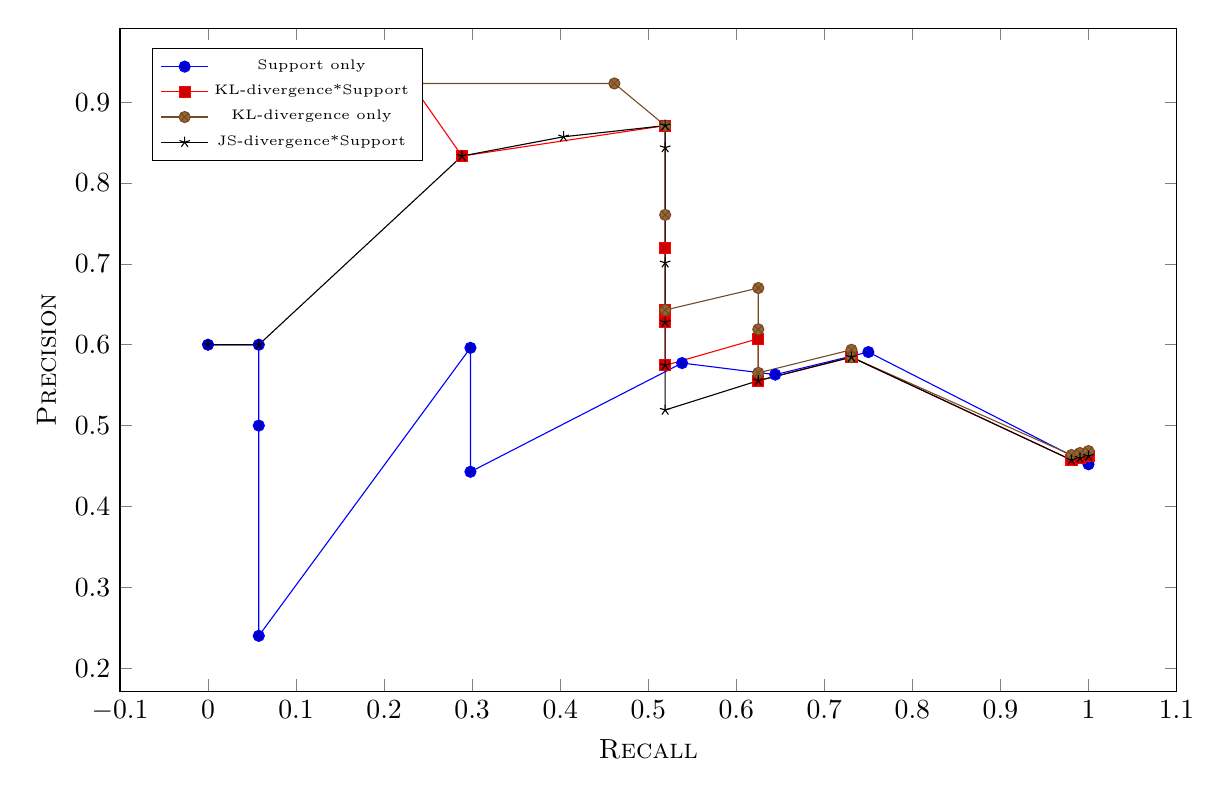
\begin{tikzpicture}[scale=1.0]
  \begin{axis}[
	width=15cm, height=10cm,
	xlabel=\textsc{Recall},
	ylabel=\textsc{Precision},
        legend entries={Support only, KL-divergence*Support, KL-divergence only, JS-divergence*Support},
	legend style={legend pos=north west,font=\tiny}]
      ]
  \addplot coordinates {(0.0,0.6) (0.05769231,0.6) (0.05769231,0.5) (0.05769231,0.24) (0.2980769 ,
0.5961539) (0.2980769,0.4428571) (0.5384616,0.5773196) (0.6442308,0.5630252) (0.75,0.5909091) (1 ,
0.4521739)};

  \addplot coordinates { (0.0,0.9230769) (0.2307692,0.9230769) (0.2884615,0.8333333) (0.5192308,0.8709678)
(0.5192308,0.72) (0.5192308,0.6428571) (0.5192308,0.627907) (0.5192308,0.5744681) (0.625,0.6074766)
(0.625,0.5555556) (0.7307692,0.5846154) (0.9807692,0.4573991) (0.9903846,0.4598214) (1.0,0.4622222)};

\addplot coordinates {(0.0,0.9230769) (0.2307692,0.9230769) (0.4615385,0.9230769) (0.5192308,0.8709678)
(0.5192308,0.7605634) (0.5192308,0.6428571) (0.625,0.6701031) (0.625,0.6190476) (0.625,0.5652174) (
0.7307692,0.59375) (0.7307692,0.5846154) (0.9807692,0.4636364) (0.9903846,0.4660633) (1.0,0.4684685)};

  \addplot coordinates {(0.0,0.6) (0.05769231,0.6) (0.2884615,0.8333333) (0.4038461,0.8571429) (0.5192308
, 0.8709678) (0.5192308,0.84375) (0.5192308,0.7012987) (0.5192308,0.627907) (0.5192308,0.5744681) (
0.5192308,0.5192308) (0.625,0.5555556) (0.7307692,0.5846154) (0.9807692,0.4573991) (0.9903846 ,
0.4598214) (1.0,0.4622222)};
  \end{axis}
  \end{tikzpicture}
\end{figure}


\begin{figure}
%\begin{minipage}{1\linewidth}\centering
 \caption{Runtime-LearnedRules}
 \centering
 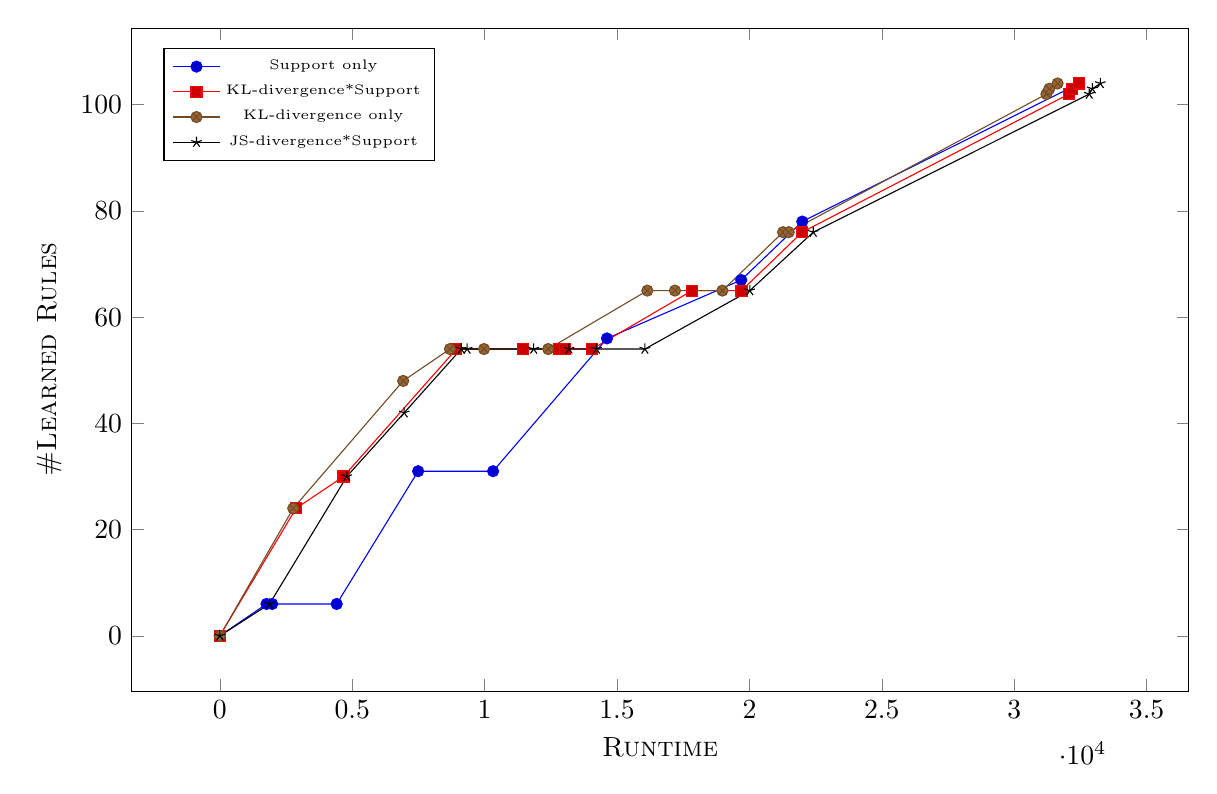
\begin{tikzpicture}
  \begin{axis}[
	width=15cm, height=10cm,
	xlabel=\textsc{Runtime},
	ylabel=\textsc{\#Learned Rules},
        legend entries={Support only, KL-divergence*Support, KL-divergence only, JS-divergence*Support},
	legend style={legend pos=north west,font=\tiny}]
      ]
  \addplot coordinates { (0.0,0.0) (1762,6) (1976,6) (4413,6) (7488,31) (10319,31) (14620,56) (
19691,67) (21995,78) (32452,104)};

  \addplot coordinates {(0.0,0.0) (2877,24) (4672,30) (8934,54) (11447,54) (12813,54) (13033,54)
(14057,54) (17836,65) (19703,65) (21991,76) (32064,102) (32173,103) (32449,104)};

  \addplot coordinates {(0.0,0.0) (2772,24) (6923,48) (8690,54) (9977,54) (12400,54) (16145,65)
(17187,65) (18979,65) (21270,76) (21483,76) (31215,102) (31324,103) (31637,104)};

  \addplot coordinates {(0.0,0.0) (1877,6) (4795,30) (6962,42) (9116,54) (9337,54) (11852,54) (
13187,54) (14225,54) (16052,54) (20014,65) (22411,76) (32833,102) (32949,103) (33251,104
)};
  \end{axis}
  \end{tikzpicture}
 % \end{minipage}
\end{figure}

















\begin{comment}
 \begin{figure}
\caption{Lattices with 3 levels}
\centering
\begin{tikzpicture}[scale=1.0]
 \begin{axis}[
	width=15cm, height=10cm,
        xlabel=\textsc{\#Nodes per lattice level},
        ylabel=\textsc{Time to build lattice ($ms$)}
    ]
\addplot coordinates {(5,2165) (10,4337) (15,6723) (20,8860) (30,11969) (40,14626) (50,21288) (60,22329) (70,24577)
(80,25387) (90,27539) (100,30210)};
\addplot coordinates {(5, 235) (10,748) (15, 1317) (20, 1590) (30, 1890) (40, 2482) (50, 3182) (60, 3474) (70, 4020)
(80, 4911) (90,5982) (100,6684)};
\end{axis}
\end{tikzpicture}
\end{figure}

\begin{figure}
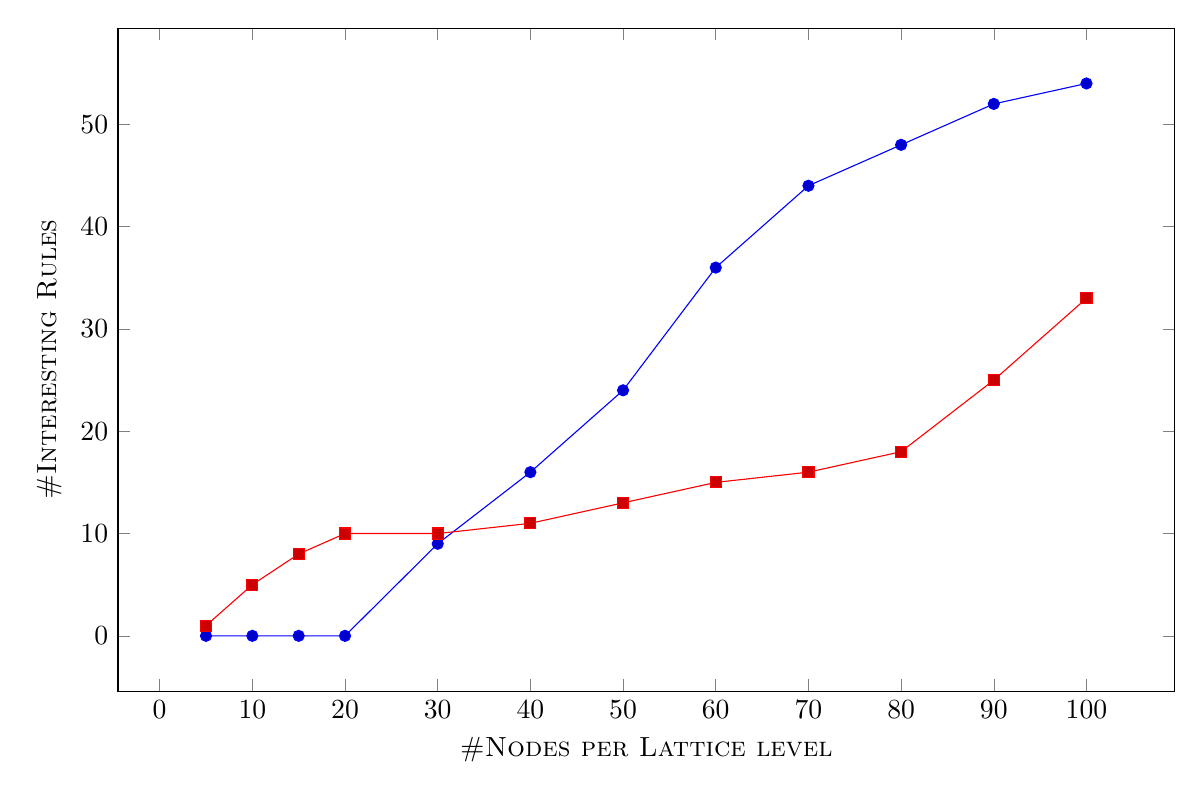
\begin{tikzpicture}[scale=1.0]
 \begin{axis}[
	width=15cm, height=10cm,
        xlabel=\textsc{\#Nodes per Lattice level},
        ylabel=\textsc{\#Interesting Rules}
    ]
\addplot coordinates {(5,0.0) (10,0.0) (15,0.0) (20, 0) (30, 9) (40,16) (50,24) (60,36) (70,44) (80,48) (90,52)
(100,54)};
\addplot coordinates {(5,1.0) (10,5) (15,8) (20,10) (30,10) (40,11) (50,13) (60,15) (70,16) (80,18) (90,25) (100,33)};
\end{axis}
\end{tikzpicture}
\end{figure}


\begin{figure}
 \caption{Lattice with 4 levels}
 \centering
 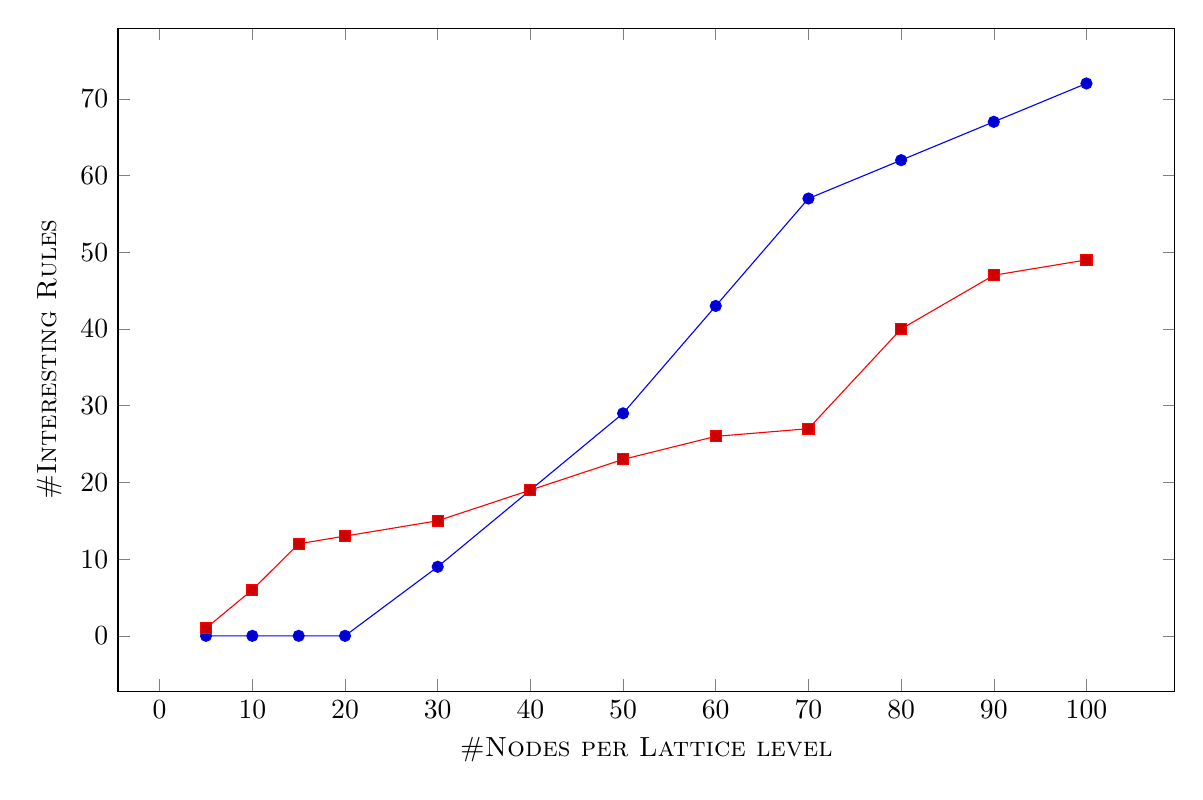
\begin{tikzpicture}[scale=1.0]
  \begin{axis}[
	  width=15cm, height=10cm,
	  xlabel=\textsc{\#Nodes per Lattice level},
	  ylabel=\textsc{\#Interesting Rules}
      ]
  \addplot coordinates {(5,0.0) (10,0.0) (15, 0) (20, 0) (30, 9) (40,19) (50,29) (60,43) (70,57) (80,62) (90,67)
(100,72)};
  %(110,75) (120,79) (130,84) (140,88) (150,94) (200,122) (250,159) (300,178) (350,200) (400,214) (450,231) (500,242)};
  \addplot coordinates {(5,1.0) (10,6) (15,12) (20,13) (30,15) (40,19) (50,23) (60,26) (70,27) (80,40) (90,47)
(100,49)};
  %(110,) (120,) (130,) (140,) (150,) (200,) (250,) (300,) (350,) (400,) (450,) (500,)};
  \end{axis}
  \end{tikzpicture}
\end{figure}

\begin{figure}
  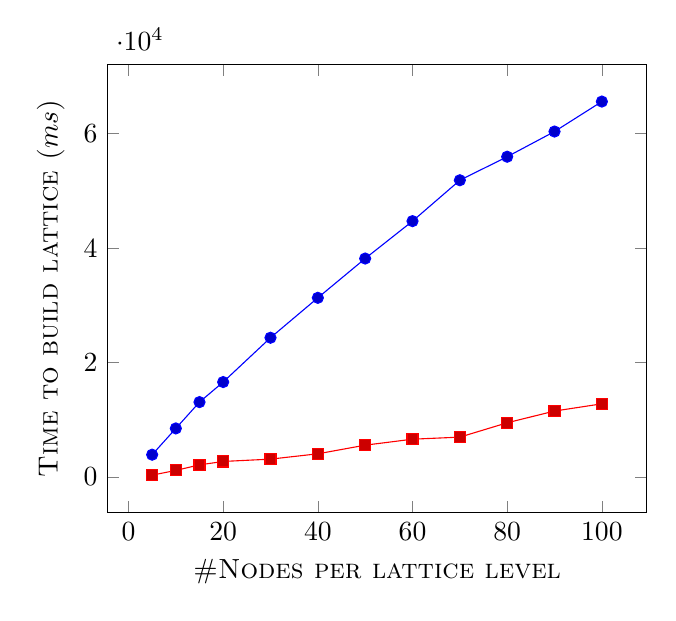
\begin{tikzpicture}[scale=1.0]
  \begin{axis}[
	  xlabel=\textsc{\#Nodes per lattice level},
	  ylabel=\textsc{Time to build lattice ($ms$)}
      ]
  \addplot coordinates {(5,3905) (10,8496) (15,13097) (20,16601) (30,24348) (40,31322) (50,38189) (60,44724) (70,51869)
  (80,55981) (90,60382) (100,65622)};
% (110,75) (120,79) (130,84) (140,88) (150,94) (200,122) (250,159) (300,178)  (350,200) (400,214) (450,231) (500,242)};
  \addplot coordinates {(5, 330) (10,1161) (15, 2128) (20, 2722) (30, 3130) (40, 4060) (50, 5571) (60, 6613) (70, 6976)
  (80, 9483) (90,11534) (100,12795)};
% (110,) (120,) (130,) (140,) (150,) (200,) (250,) (300,) (350,) (400,) (450,) (500,)};
  \end{axis}
  \end{tikzpicture}
\end{figure}
\end{comment}



